\chapter{Tinjauan Pustaka}

\section{\textit{Voice Assistant}}

\textit{Voice assistant}, atau asisten suara, merupakan turunan dari \textit{virtual assistant}. \textit{Virtual assistant} terdiri dari dua kata, \textit{virtual} dan \textit{assistant}. \textit{Assistant} atau asisten, menurut Kamus Besar Bahasa Indonesia (KBBI) adalah orang yang bertugas membantu orang lain dalam melaksanakan tugas profesional \parencite{kbbi}. Lalu \textit{virtual}, menurut KBBI, adalah tampil atau hadir dengan menggunakan perangkat lunak komputer. Jadi, dapat disimpulkan bahwa \textit{virtual assistant} adalah orang, dalam hal ini \textit{artificial intelligence}, yang hadir dalam sebuah perangkat tertentu, bertugas untuk membantu orang lain dalam melaksanakan tugas. \textit{Virtual assistant} kadang sering disebut dengan \textit{chatbot} karena kemampuannya dalam melakukan percakapan dengan penggunanya \parencite{tech2005imbot}. \textit{Virtual assistant} memiliki beberapa jenis interaksi selain melalui suara, seperti teks atau gambar. Salah satu jenis interaksi yang akan menjadi fokus dalam Tugas Akhir adalah interaksi melalui suara, atau disebut juga dengan asisten suara.

Gambaran besar mengenai \textit{voice assistant} dapat dilihat pada Gambar \ref{fig:slu_early} yang merupakan alur proses pemahaman bahasa terucap atau \textit{spoken language understanding} (SLU) \parencite{tur2011spoken}. Suara yang diberikan pengguna diterima oleha pengenal suara atau \textit{speech recognition} dan diubah menjadi sebuah teks. Pengenalan suara menggunakan pengetahuan akustik, leksikal, dan bahasa yang tersimpan dalam sumber pengetahuan (\textit{knowledge source}) untuk pengenalan suara itu sendiri. Pengetahuan tersebut diterjemahkan oleh pengendali atau \textit{control} sehingga dapat digunakan oleh pengenalan suara.

Teks yang berasal dari pengenal suara diberikan ke pemahaman bahasa alami atau \textit{natural language understanding} (NLU) untuk menemukan maksud pengguna menggunakan teks tersebut. Seperti pada pengetahuan suara, pemahaman bahasa alami juga memiliki sumber pengetahuan tersendiri untuk menyimpan pengetahuan mengenai sintaksis dan semantik yang diterjemahkan oleh pengendali untuk menciptakan hipotesis maksud dari sebuah kalimat. Setelah asisten dapat mengetahui maksud dari apa yang diucapkan oleh pengguna, asisten kemudian melakukan serangkaian aksi yang berkaitan dengan maksud ucapan pengguna tersebut. Bagian \textit{voice assistant} yang menjadi fokus dalam pengerjaan Tugas Akhir adalah bagian NLU.
\begin{figure}[ht]
	\centering
	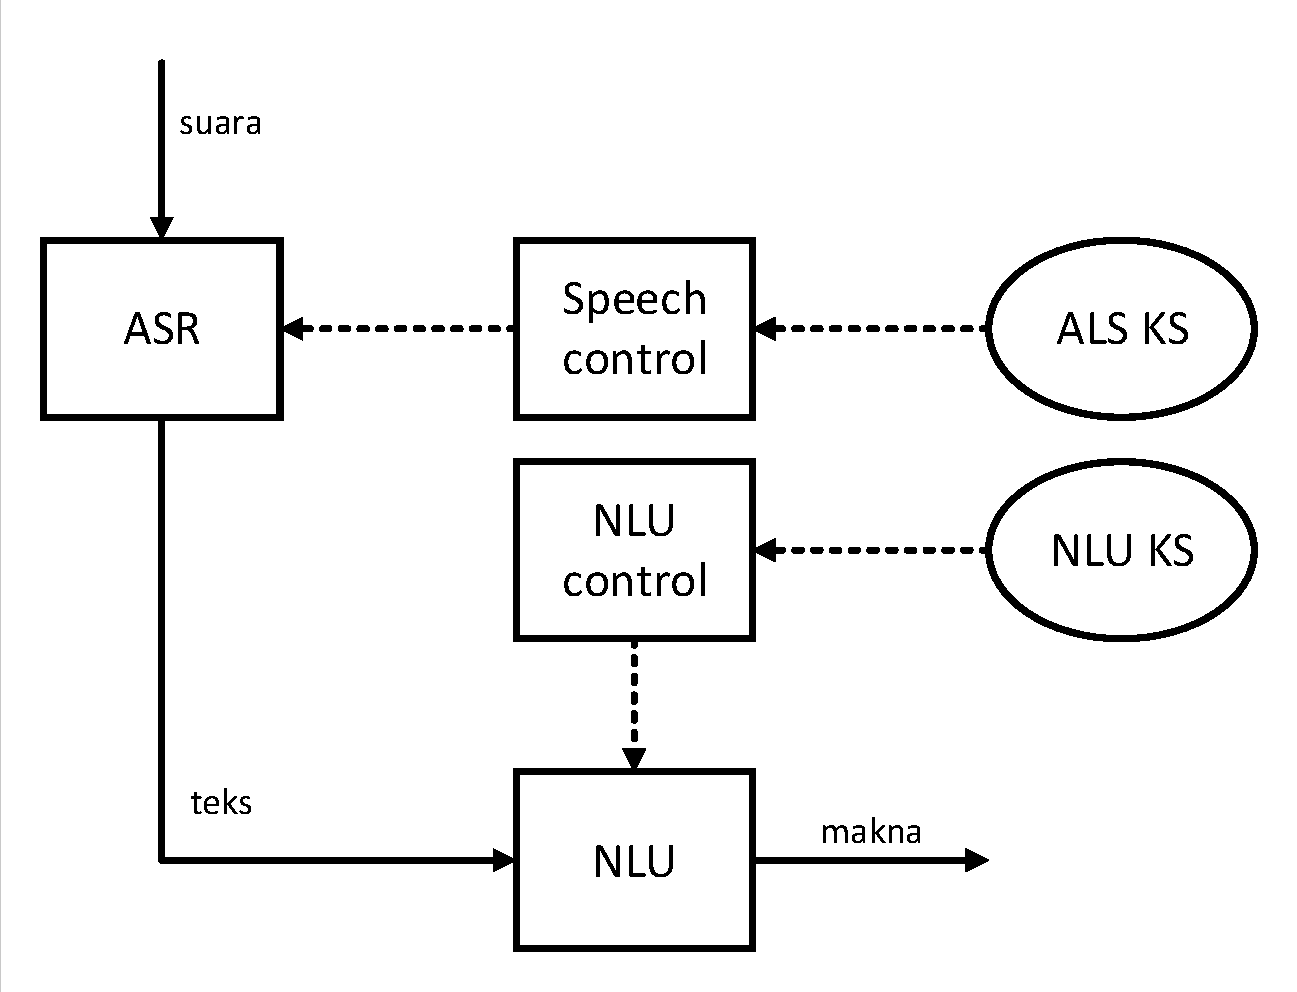
\includegraphics[width=0.6\textwidth, trim=2 2 2 2, clip]{resources/2/early_slu.pdf}
	\caption{Alur proses \textit{spoken language understanding} \parencite{tur2011spoken}}
	\label{fig:slu_early}
\end{figure}

\subsection{\textit{Natural Language Understanding} (NLU)}

NLU merupakan ranah dalam linguistik komputasional yang didedikasikan untuk memahami bahasa alami \parencite{harris2004voice}. Gartner \parencite{gartnernatural} mendefinisikan NLU sebagai pemahaman komputer terhadap struktur dan makna dari bahasa manusia sehingga pengguna dapat berinteraksi dengan komputer menggunakan bahasa yang digunakan oleh pengguna. Dari kedua definisi tersebut, dapat disimpulkan bahwa NLU merupakan bagian komputasional untuk memahami bahasa yang sering digunakan oleh manusia.

Perlu diperhatikan bahwa komputer berusaha untuk memahami bahasa manusia sehingga komputer perlu memiliki pengetahuan yang dasarnya dimiliki oleh manusia dalam berbahasa. James Allen \parencite{allen1995natural} menyebutkan bahwa terdapat enam bentuk pengetahuan yang diketahui dan dipelajari oleh manusia. Pengetahuan tersebut didefinisikan sebagai berikut:
\begin{enumerate}
	\item pengetahuan fonetik dan fonologi, yaitu tentang cara suara diubah menjadi susunan kata-kata. Dalam ilmu komputer, pengetahuan ini diatasi dengan menggunakan \textit{speech recognition};
	\item pengetahuan morfologi, yaitu tentang cara sebuah kata disusun dari beberapa morfem, seperti kata “terabaikan” disusun oleh tiga morfem, yaitu “ter-”, “abai”, dan “-kan”;
	\item pengetahuan sintaktis,yaitu tentang cara kata-kata disusun menjadi sebuah kalimat yang benar menurut tata bahasa;
	\item pengetahuan semantik, yaitu tentang kata-kata disusun untuk membentuk makna dari sebuah kalimat;
	\item pengetahuan pragmatik, yaitu tentang sebuah kalimat diartikan jika digunakan dalam konteks yang berbeda; dan
	\item pengetahuan dunia, yaitu tentang memahami pengetahuan umum yang dipahami juga oleh pengguna untuk menjaga percakapan berjalan dengan semestinya.
\end{enumerate}

Pengetahuan yang dicakup dalam NLU saja adalah pengetahuan sintaksis, semantik, dan pragmatik. Terdapat empat kategori pendekatan yang digunakan untuk membangun NLU \parencite{yao2017four}, yaitu:
\begin{enumerate}
	\item pendekatan distribusi, yaitu penggunaan taktik statistik skala besar dengan pembelajaran mesin (\textit{machine learning});
	\item pendekatan berdasarkan rangka, yaitu penggunaan struktur data untuk representasi situasi yang sering terjadi;
	\item pendekatan model teoritis, yaitu menganggap sebuah kalimat selalu mengacu kepada yang ada di dunia dan bagian-bagian kalimat dapat digabungkan untuk membentuk sebuah makna; dan
	\item pendekatan pembelajaran interaktif, yaitu penggunaan  lingkungan interaktif antara manusia dengan komputer.
\end{enumerate}

Pendekatan yang menjadi fokus dalam pengerjaan Tugas Akhir adalah pendekatan distribusi, yang mana menggunakan pembelajaran mesin.

\subsection{Pembelajaran Mesin}

Tom Mitchell \parencite{mitchell1997machine} mendefinisikan pembelajaran mesin sebagai sebuah program komputer yang dirancang untuk belajar dari pengalaman \textit{E} dengan acuan berupa kelas tugas-tugas \textit{T} dan pengukuran kinerja \textit{P}, kinerja pada suatu tugas \textit{T}, yang diukur dengan \textit{P}, dan diperbaiki dengan pengalaman \textit{E}. Sebagai contoh, program menjalankan tugas (\textit{T}) untuk bermain dam. Ukuran program tersebut (\textit{P}) adalah persentase sebuah program menang dalam permainan dam. Untuk meningkatkan persentase tersebut, program harus belajar dari pengalaman (\textit{E}) berupa permainan yang telah dilakukan melawan program itu sendiri.

Terdapat tiga kategori umum untuk pembelajaran mesin berdasarkan cara belajar \parencite{ray2015essentials}. Tiga kategori tersebut adalah pembelajaran terkontrol, pembelajaran tidak terkontrol, dan pembelajaran penguatan. Algoritme pembelajaran terkontrol mengandung variabel terikat atau keluaran yang akan diprediksi jika diberikan sekumpulan variabel bebas sehingga membentuk fungsi yang dapat memetakan masukan menjadi keluaran yang diinginkan. Algoritme pembelajaran tidak terkontrol tidak memiliki variabel terikat untuk diprediksi sehingga algoritme harus mengelompokkan sendiri. Pembelajaran tidak terkontrol biasa digunakan untuk pengelompokan populasi ke dalam kelompok yang berbeda. Terakhir, algoritme pembelajaran penguatan menggunakan teknik coba-coba sebagai metode pembelajaran sehingga dapat membentuk program dengan keputusan yang spesifik. Algoritme yang menjadi fokus dalam Tugas Akhir adalah algoritme pembelajaran terkontrol, misalnya \textit{Naive Bayes}, \textit{Decision Tree}, \textit{Support Vector Machine} (SVM), dan \textit{Artificial Neural Network} (ANN).

\subsection{\textit{Artificial Neural Network} (ANN)}

Menurut Caudill \parencite{caudill1987neural}, ANN adalah sistem komputasi yang memiliki elemen-elemen pemrosesan sederhana yang saling terhubung, yang mana dapat memproses informasi dengan respon keadaan dinamisnya kepada masukan dari luar. Rupa ANN yang paling dasar dapat dilihat pada Gambar \ref{fig:ann} yang hanya terdiri dari tiga bagian lapisan, yaitu lapisan masukan, lapisan tersembunyi, dan lapisan keluaran. Satu lapisan terdiri dari kumpulan beberapa neuron yang digunakan sebagai fungsi aktivasi, dan neuron antarlapisan dihubungkan dengan bobot yang didefinisikan saat latihan berlangsung.
\begin{figure}[ht]
	\centering
	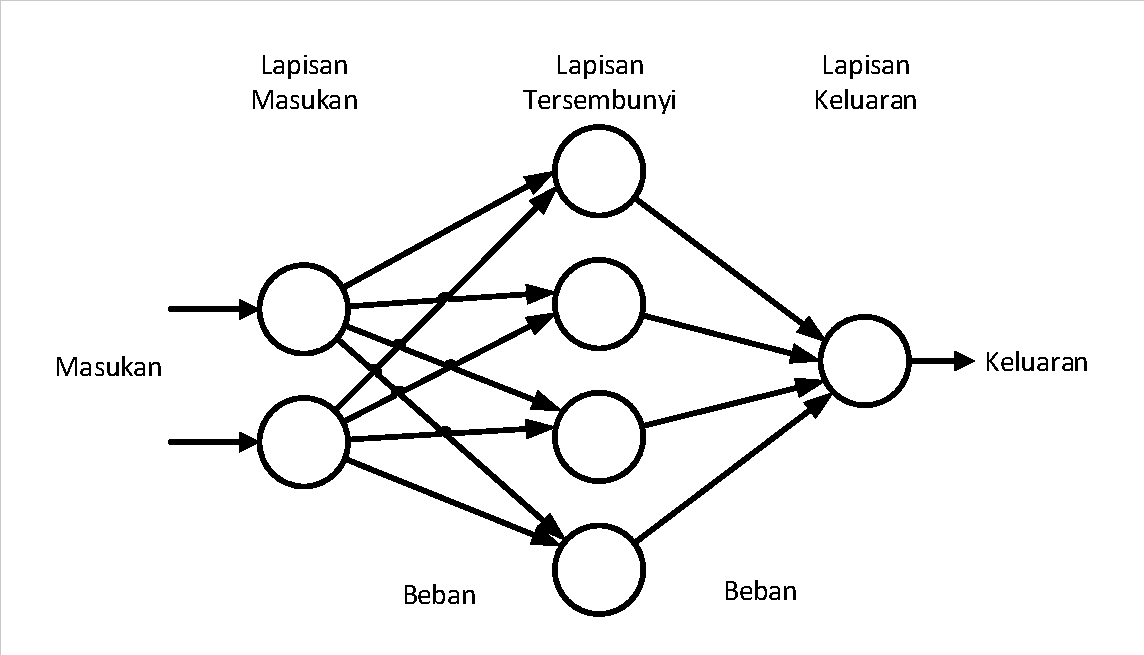
\includegraphics[width=0.9\textwidth, trim=2 2 2 2, clip]{resources/2/ann.pdf}
	\caption{Rupa dasar ANN \parencite{caudill1987neural}}
	\label{fig:ann}
\end{figure}

\subsection{\textit{Word Embedding}}

Salah satu penerapan ANN untuk NLU adalah operasi \textit{word embedding}, yaitu representasi yang telah belajar untuk teks dengan kata-kata yang memiliki makna yang sama saling berdekatan satu sama lain \parencite{brownlee2017what}. Terdapat dua cara untuk menggunakan \textit{word embedding}, yaitu dengan mempelajari \textit{embedding} baru atau menggunakan kembali \textit{embedding} yang sudah ada. Cara yang akan digunakan dalam fokus pengerjaan Tugas Akhir adalah dengan mempelajari \textit{embedding} baru.

Cara \textit{embedding} belajar dapat dilihat pada Gambar \ref{fig:cbow}, yang menggambarkan proses pembelajaran \textit{embedding} dengan teknik kantong kata berlanjut atau \textit{continuous bag-of-words} (CBOW) \parencite{Rong2014word2vecPL}. Sebuah kata diubah terlebih dahulu menjadi kantong kata yang merupakan vektor dengan ukuruan sejumlah kata dalam kamus $V$. Kantong kata dibentuk dengan teknik \textit{one-hot encoding}, yaitu vektor diisi nilai 1 untuk kata yang sesuai dan 0 untuk kata yang tidak sesuai. Kantong kata yang telah dibentuk dimasukkan ke lapisan masukan ANN dengan besar lapisan tersembunyi sejumlah $N$. Antara lapisan masukan dengan lapisan tersembunyi berupa matriks dua dimensi $W$, begitu pula antara lapisan tersembunyi dengan lapisan keluaran yaitu $W'$.
\begin{figure}[ht]
	\centering
	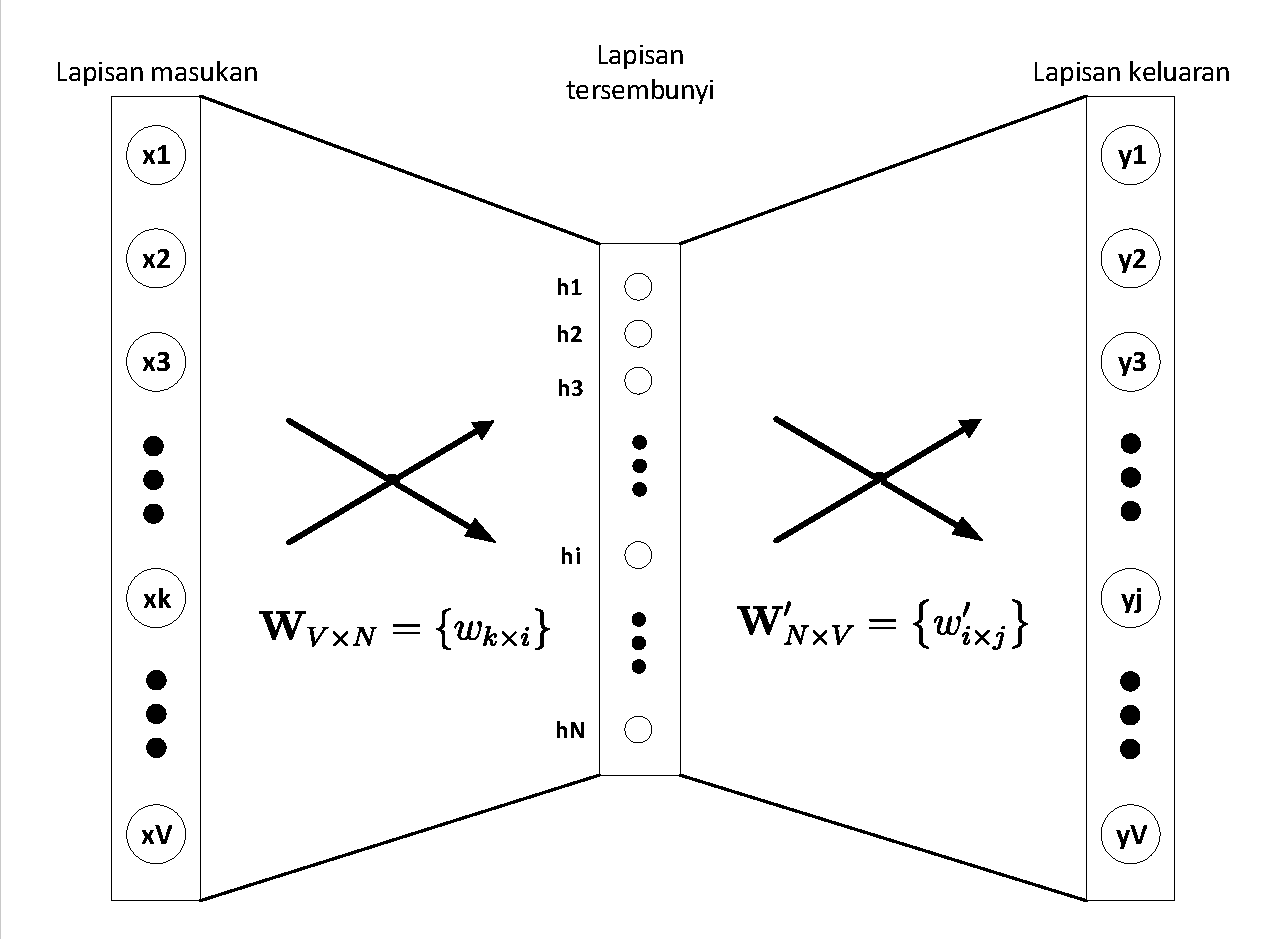
\includegraphics[width=0.8\textwidth, trim=2 2 2 2, clip]{resources/2/cbow.pdf}
	\caption{Model sederhana CBOW \parencite{Rong2014word2vecPL}}
	\label{fig:cbow}
\end{figure}

Namun, terdapat permasalahan terhadap kamus yang dibentuk, salah satunya adalah kata yang akan diubah menjadi indeks harus ada di dalam kamus. Meskipun dalam kamus tersebut terdapat indeks khusus yang menyatakan kata yang tidak diketahui, kata tidak dapat diubah menjadi indeks kata yang tidak diketahui. Oleh karena itu, diperlukan salah satu fungsi yang dipasangkan sebelum menjadi masukan pada lapisan \textit{embedding}. Fungsi tersebut harus dapat menemukan kata dalam kamus yang mirip dengan kata yang sedang diubah menjadi indeks. Metode yang dapat digunakan untuk mencari kata yang mirip dalam kamus adalah dengan menggunakan metode jarak perbedaan antara kedua kata.

\subsection{Jarak Perubahan}

Jarak perubahan adalah jumlah operasi perubahan terkecil yang dibutuhkan untuk mengubah teks, misal teks A menjadi teks B \parencite{schutze2008introduction}. Terdapat beberapa variasi metode untuk mencari jarak perubahan kedua teks. Dengan kemampuan dalam menebak kata yang mirip, jarak perubahan dapat digunakan untuk melakukan normalisasi sebuah teks. Normalisasi menurut KBBI \parencite{kbbi} adalah tindakan menjadikan normal kembali. Dengan definisi tersebut, dapat disimpulkan bahwa normalisasi teks adalah tindakan untuk menjadikan teks yang berantakan kembali normal, dalam hal ini teks yang sesuai dengan bahasa yang baku.

\section{Normalisasi Teks}

Terdapat sebuah penelitian terkait normalisasi teks, yaitu penelitian normalisasi teks dalam suntingan media sosial Twitter, atau disebut juga dengan \textit{tweet}, untuk bahasa Indonesia yang memiliki karakteristik berupa kata yang disingkat \parencite{saragih2017normalisasi}. Penelitian ini bertujuan untuk menerapkan algoritme penghitungan jarak dua kata dan membuat fungsi untuk normalisasi kata yang tidak baku menjadi kata baku. Keseluruhan pembangunan tersebut dilakukan dengan menggunakan bahasa pemrograman R.

Penelitian dilakukan dengan menggunakan fungsi \textit{stringdist} pada bahasa R. Fungsi \textit{stringdist} memiliki dua parameter wajib, yaitu kata pertama dan kata kedua, serta delapan parameter opsional, salah satunya adalah pilihan algoritme pengukuran jarak. Fungsi \textit{stringdist} memiliki 10 variasi algoritme pengukuran jarak sebagai berikut:
\begin{enumerate}
	\item jarak \textit{optimal string alignment} (\textit{osa});
	\item jarak Levenshtein (\textit{lv});
	\item jarak \textit{full Damerau-Levenshtein} (\textit{dl});
	\item jarak Hamming (\textit{hamming});
	\item jarak \textit{longest common substring} (\textit{lcs});
	\item jarak \textit{q-gram} (\textit{qgram});
	\item jarak \textit{cosine} (\textit{cosine});
	\item jarak Jaccard (\textit{jaccard});
	\item jarak Jaro-Winker (\textit{jw}); dan
	\item jarak \textit{Soundex} (\textit{soundex}).
\end{enumerate}

\subsection{Alur Proses Normalisasi Teks}

Berdasarkan \parencite{saragih2017normalisasi} alur proses normalisasi teks yang dibangun dapat dilihat pada Gambar \ref{fig:flow_saragih}. Alur tersebut merupakan alur untuk tiap kata yang terdapat dalam \textit{tweet} berbahasa Indonesia. Proses membutuhkan dua jenis kamus, yaitu kamus kata tidak baku beserta perbaikannya dan kamus kata baku. Kamus kata tidak baku disusun secara manual, yaitu dengan menentukan kata yang termasuk kata tidak baku bahasa Indonesia, baik kata dari bahasa daerah, bahasa gaul, atau bahasa asing, lalu menentukan kata baku yang merupakan makna dari kata tidak baku tersebut. Untuk kamus kata baku, terdapat tiga jenis kamus yang digunakan, yaitu kamus kata baku dari KBBI diambil dari sebuah perangkat lunak, kamus yang diambil dari korpus arsip situs web Kompas tahun 2012, serta kamus dari korpus Kompas yang telah disaring sehingga hanya mengandung kata yang sesuai dalam KBBI.
\begin{figure}[ht]
	\centering
	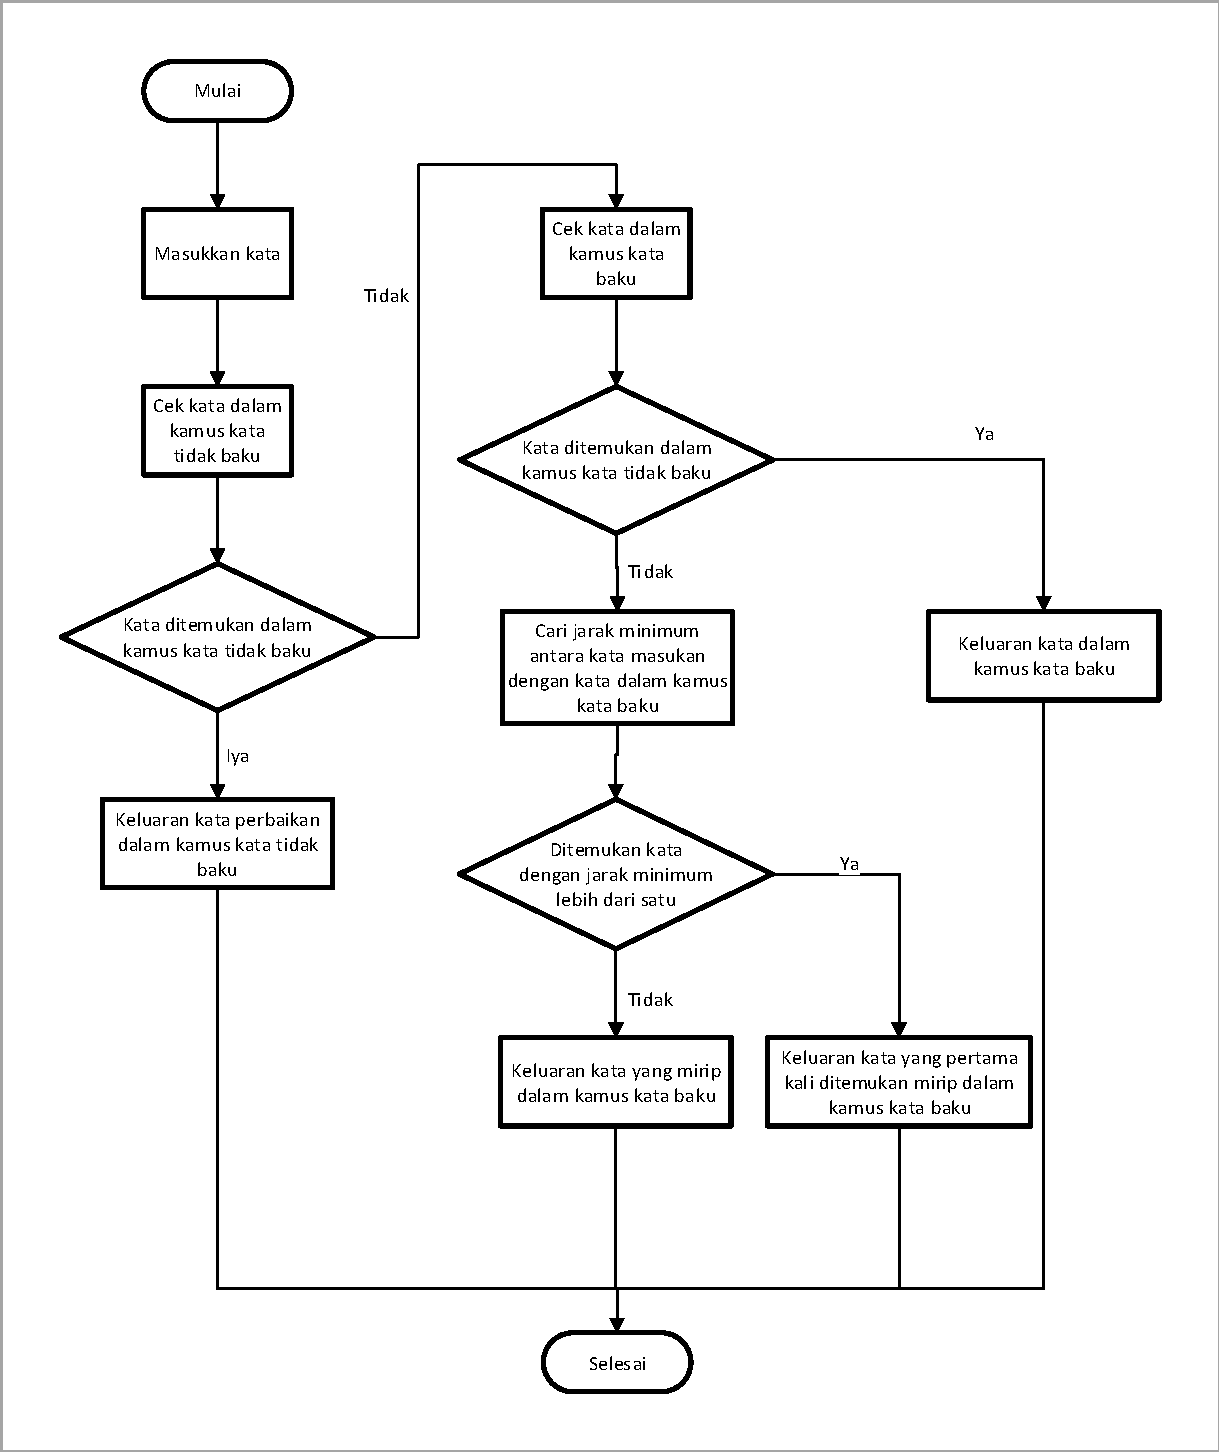
\includegraphics[width=0.8\textwidth, trim=2 2 2 2, clip]{resources/2/flow_saragih.pdf}
	\caption{Alur proses normalisasi teks \parencite{saragih2017normalisasi}}
	\label{fig:flow_saragih}
\end{figure}

Proses normalisasi teks dimulai dari menerima kata masukan, lalu dilanjutkan dengan memeriksa kata masukan dengan kamus kata tidak baku. Jika kata masukan terdapat dalam kamus kata tidak baku, maka kata baku yang menjadi perbaikannya dipilih menjadi kata luaran. Jika tidak ditemukan, proses berlanjut dengan memeriksa kata masukan dengan kamus kata baku. Jika ditemukan, maka kata yang dipilih dalam kamus kata baku tersebut menjadi kata luaran. Jika tidak, proses dilanjutkan dengan mencari kata yang mirip di dalam kamus kata baku dengan menerapkan fungsi \textit{stringdist}.

Fungsi \textit{stringdist} digunakan untuk mencari jarak minimum antara kata masukan dan kata dalam kamus kata baku. Setelah itu, jarak minimum tersebut digunakan untuk mencari kumpulan kata dalam kamus kata baku. Jika hanya ditemukan satu kata dalam kamus, kata tersebut yang terpilih menjadi kata luaran. Jika ditemukan lebih dari satu, kata dalam kamus yang dipilih menjadi kata luaran adalah kata yang pertama kali ditemukan. Metode tersebut dipilih dengan mempertimbangkan bahwa kata dalam kamus yang berasal dari korpus Kompas diurut berdasarkan frekuensi kemunculan kata tersebut.

\subsection{Evaluasi Normalisasi Teks}

Evaluasi proses normalisasi teks dilakukan dengan memasukkan 200 kata tidak baku yang diambil dari kumpulan \textit{tweet} berbahasa Indonesia yang telah diolah sebelumnya. Tabel \ref{tbl:ipb_tweet} menunjukkan 15 kata pertama yang digunakan untuk evaluasi. Evaluasi dilakukan hanya pada proses yang membutuhkan fungsi \textit{stringdist}. Sebanyak 10 algoritme pengukuran jarak yang tersedia dalam fungsi \textit{stringdist} dievaluasi dengan mengukur persentase akurasi terhadap 200 kata \textit{tweet} tidak baku. Penghitungan persentase akurasi dilakukan sebagai berikut:
\begin{equation*}
	\text{Persentase akurasi}=\frac{\text{x}}{y} \times 100\%
\end{equation*}
\noindent
dengan $x$ adalah jumlah kata yang tepat, yaitu kata tersebut sesuai dengan kata luaran yang diharapkan, dan $y$ adalah jumlah seluruh kata yang diuji, yaitu 200 kata.
\begin{table}[ht]
	\captionsetup{justification=justified,singlelinecheck=false}
	\caption{Lima belas (15) kata pertama yang digunakan untuk evaluasi \parencite{saragih2017normalisasi}}
    \label{tbl:ipb_tweet}
    \centering
	\begin{tabular}{|c|c|c|}
		\hline
		\multicolumn{3}{|c|}{\textbf{Kata uji dari \textit{tweet}}} \\ \hline
		\textit{adalh} & \textit{agr} & \textit{asem} \\ 
		\textit{akhirny} & \textit{ambl} & \textit{baek} \\ 
		\textit{akn} & \textit{and} & \textit{baikk} \\ 
		\textit{aktf} & \textit{apalg} & \textit{bban} \\ 
		\textit{adlh} & \textit{apkh} & \textit{bdan} \\ \hline
	\end{tabular}
\end{table}

Beberapa kelemahan dimiliki oleh dua kamus baku yaitu yang berasal dari KBBI dan korpus Kompas tanpa penyaringan. Kamus kata baku dari KBBI memiliki masalah dengan pengubahan menjadi kata baku yang jarang digunakan oleh masyarakat. Sebagai contoh, kata "\textit{asem}" yang biasa diartikan sebagai "asam" justru diartikan sebagai "rasem" yang berarti bunga tandan. Untuk menangani masalah tersebut, diperlukan kamus dengan urutan berupa frekuensi sebuah kata dipakai atau muncul, yang mana merupakan karakteristik dari kamus berdasarkan korpus Kompas. Namun, kamus korpus Kompas memiliki kelemahan, yaitu beberapa perbaikan kata keluarannya termasuk dalam kata tidak baku, seperti "\textit{entr}" menjadi "\textit{center}" yaitu kata bahasa Inggris dari "tengah", "\textit{ckp}" berubah menjadi "\textit{kpk}" yang kemungkinan mengacu kepada singkatan dari Komisi Pemberantasan Korupsi, dan lain-lain. Solusi yang diterapkan untuk masalah yang terdapat pada kedua kamus adalah dengan menggunakan kamus dari korpus Kompas, namun disaring sehingga kamus hanya mengandung kata-kata yang baku menurut kamus KBBI.

Hasil evaluasi ketiga pengujian disajikan dalam Tabel \ref{tbl:ipb_eval_1}, Tabel \ref{tbl:ipb_eval_2}, dan Tabel \ref{tbl:ipb_eval_3}. Semua tabel menunjukkan persentase dari 10 algoritme pengukuran jarak dalam fungsi \textit{stringdist}. Tabel \ref{tbl:ipb_eval_1}, yaitu pengujian dengan kamus dari KBBI, menunjukkan hanya dua metode saja yang dapat mencapai persentase akurasi lebih dari 50 persen. Tabel \ref{tbl:ipb_eval_2}, yaitu hasil pengujian dengan kamus korpus Kompas, menunjukkan peningkatan yang signifikan sehingga sudah ada 5 metode dengan persentase akurasi lebih dari 50 persen, dua diantaranya sudah melebihi 60 persen. Terakhir Tabel \ref{tbl:ipb_eval_3}, yaitu hasil pengujian dengan kamus Korpus Kompas yang telah disaring, menunjukkan peningkatan persentase akurasi namun tidak setinggi perubahan pada Tabel \ref{tbl:ipb_eval_2}. Lalu, terdapat satu metode yang mengalami penurunan persentase akurasi, yaitu algoritme jarak Jaccard. Persentase akurasi semua tabel didominasi oleh metode jarak LCS.
\begin{table}[H]
	\captionsetup{justification=justified,singlelinecheck=false}
	\caption{Pengujian 10 metode \textit{stringdist} dengan menggunakan kamus dari KBBI}
    \label{tbl:ipb_eval_1}
    \centering
	\begin{tabular}{|c|c|c|r|}
		\hline
		No & Metode & Jumlah kata benar & \multicolumn{1}{c|}{Akurasi} \\ \hline
		1 & \textit{osa} & 74 & 37\% \\
		2 & \textit{lv} & 75 & 37,5\% \\
		3 & \textit{dl} & 75 & 37,5\% \\
		4 & \textit{hamming} & 17 & 8,5\% \\
		5 & \textit{lcs} & 100 & 50\% \\
		6 & \textit{qgram} & 35 & 17,5\% \\
		7 & \textit{cosine} & 46 & 23\% \\
		8 & \textit{jaccard} & 36 & 18\% \\
		9 & \textit{jw} & 111 & 55,5\% \\
		10 & \textit{soundex} & 9 & 4,5\% \\ \hline
	\end{tabular}
\end{table}

\begin{table}[H]
	\captionsetup{justification=justified,singlelinecheck=false}
	\caption{Pengujian 10 metode \textit{stringdist} dengan menggunakan kamus dari korpus Kompas}
    \label{tbl:ipb_eval_2}
    \centering
	\begin{tabular}{|c|c|c|r|}
		\hline
		No & Metode & Jumlah kata benar & \multicolumn{1}{c|}{Akurasi} \\ \hline
		1 & \textit{osa} & 116 & 58\% \\
		2 & \textit{lv} & 116 & 58\% \\
		3 & \textit{dl} & 116 & 58\% \\
		4 & \textit{hamming} & 24 & 12\% \\
		5 & \textit{lcs} & 133 & 66,5\% \\
		6 & \textit{qgram} & 82 & 41\% \\
		7 & \textit{cosine} & 87 & 43,5\% \\
		8 & \textit{jaccard} & 92 & 46\% \\
		9 & \textit{jw} & 124 & 62\% \\
		10 & \textit{soundex} & 67 & 33,5\% \\ \hline
	\end{tabular}
\end{table}

\begin{table}[H]
	\captionsetup{justification=justified,singlelinecheck=false}
	\caption{Pengujian 10 metode \textit{stringdist} dengan menggunakan kamus dari korpus Kompas yang sesuai dengan KBBI}
    \label{tbl:ipb_eval_3}
    \centering
	\begin{tabular}{|c|c|c|r|}
		\hline
		No & Metode & Jumlah kata benar & \multicolumn{1}{c|}{Akurasi} \\ \hline
		1 & \textit{osa} & 119 & 59,5\% \\
		2 & \textit{lv} & 119 & 59,5\% \\
		3 & \textit{dl} & 119 & 59,5\% \\
		4 & \textit{hamming} & 24 & 12\% \\
		5 & \textit{lcs} & 138 & 69\% \\
		6 & \textit{qgram} & 89 & 44,5\% \\
		7 & \textit{cosine} & 89 & 44,5\% \\
		8 & \textit{jaccard} & 89 & 44,5\% \\
		9 & \textit{jw} & 133 & 66,5\% \\
		10 & \textit{soundex} & 71 & 35,5\% \\ \hline
	\end{tabular}
\end{table}

\subsection{Jarak \textit{Longest Common Substring} (LCS)}

Jarak LCS menghitung jarak antara dua teks dengan cara menghitung berapa kali terjadi penghapusan dan penambahan karakter suatu teks sehingga menjadi teks yang lain. Dengan kata lain, metode jarak LCS hanya mengaplikasikan dua operasi, yaitu penambahan dan pengurangan karakter. Jarak LCS yang digunakan dalam fungsi \textit{stringdist} menggunakan metode yang digunakan untuk mencari kemiripan urutan asam amino dari dua protein \parencite{needleman1970general}. Nilai jarak dengan metode LCS mengikuti persamaan:
\begin{equation} \label{eq:lcs}
	\text{lcs}_{a,b}(i,j)=\begin{cases}
		\text{max}(i,j) & \text{ jika min} (i,j)=0, \\ 
		\text{lcs}_{a,b}(i-1,j-1) & \text{ jika } a_{i}=b_{j} \text{ dan min} (i,j)\neq 0, \\
		1 + \text{min}\left \{ \text{lcs}_{a,b}(i-1,j), \text{lcs}_{a,b}(i,j-1) \right \} & \text{ jika } a_{i}\neq b_{j} \text{ dan min} (i,j)\neq 0
	\end{cases}
\end{equation}
\myequations{Persamaan Jarak \textit{Longest Common Substring} (LCS)}
\noindent
dengan $\text{lcs}_{a,b}(i,j)$ adalah jarak LCS antara $i$ karakter pertama untuk teks $a$ dengan $j$ karakter pertama untuk teks $b$.

\subsection{Kelemahan Algoritme Jarak LCS}

Hasil evaluasi menunjukkan bahwa jarak LCS menempati urutan pertama dari 10 algoritme pengukuran jarak dengan persentase akurasi tertinggi. Meskipun begitu, terdapat kekurangan analisis yang dilakukan di dalam penelitian sehingga dapat berakibat pada kesalahan pemilihan solusi. Kekurangan tersebut dapat dijelaskan apabila mengacu pada karakteristik dari algoritme jarak LCS. Sebagai contoh, analisis dalam penelitian menyatakan bahwa hasil persentase akurasi rendah pengujian pertama pada Tabel \ref{tbl:ipb_eval_1} disebabkan oleh terpilihnya kata yang jarang digunakan oleh masyarakat dan mengambil contoh berupa kata "\textit{asem}" menjadi "rasem", dan bukan "asam" seperti yang diharapkan dalam penelitian sehingga kamus kata baku KBBI diganti dengan kamus korpus Kompas. Padahal, jika ditelusur lebih jauh, terdapat beberapa keganjilan dengan analisis tersebut, yaitu:
\begin{enumerate}
	\item Alur proses normalisasi dalam penelitian menunjukkan jika terdapat lebih dari satu kata dalam kamus yang memiliki jarak minimum dengan kata masukan, maka kata yang pertama ditemukan yang akan dipilih. Kamus KBBI diurutkan berdasarkan abjad sehingga terpilihnya "rasem" daripada "asam" sangat tidak wajar. Setelah ditelusur lebih jauh, masalah "rasem" tersebut berasal dari algoritme yang digunakan, dalam hal ini algoritme salah satu metode yang dominan yaitu jarak LCS. Jarak LCS hanya memiliki dua operasi karakter, yaitu penambahan dan pengurangan \parencite{van2014stringdist}. Untuk penggantian karakter, jarak LCS menggunakan cara penambahan dan pengurangan karakter sekaligus sehingga nilai jarak untuk penggantian satu karakter bernilai 2. Jika dihubungkan dengan masalah "rasem", maka masalah tersebut menjadi lebih jelas. Masalah "rasem" terjadi karena jarak antara "\textit{asem}" dengan "rasem" lebih kecil dibandingkan dengan "\textit{asem}" dengan "asam", karena "rasem" hanya membutuhkan penambahan karakter "r" sedangkan "asam" harus mengganti karakter "e" dengan "a" yang berarti, dalam LCS, menghapus karakter "e" lalu menambah karakter "a".
	\item Penelitian tidak menunjukkan adanya masalah yang serupa dengan "rasem" dan "asam" setelah kamus dari KBBI diganti dengan kamus dari korpus Kompas sehingga bisa disimpulkan bahwa masalah tersebut telah selesai, dan menyimpulkan bahwa kepopuleran kata yang menjadi penyebab masalah seperti "rasem" dan "asam". Tapi, alur proses normalisasi teks menunjukkan bahwa fungsi \textit{stringdist} membandingkan kata masukan dengan seluruh kata yang ada di dalam kamus untuk mencari nilai jarak minimum, kemudian fungsi tersebut digunakan kembali untuk mencari kata dalam kamus dengan jarak minimum tersebut. Dengan mengacu pada kesimpulan keganjilan analisis yang pertama, hal tersebut menunjukkan bahwa kata "rasem" dapat terpilih kembali daripada "asam" meskipun berada pada urutan terakhir dalam kamus korpus Kompas, yang berarti kata tersebut tidak sering digunakan. Dengan begitu, dapat disimpulkan bahwa tidak terpilihnya kata "rasem" karena kata tersebut tidak tersedia dalam kamus korpus Kompas sehingga masalah pada pengujian pertama dengan kamus KBBI diselesaikan dengan menghapus kata dalam kamus, solusi yang juga digunakan pada masalah pengujian kedua dengan kamus korpus Kompas, bukan dengan mengurutkan kata dalam kamus sesuai seringnya kata tersebut terpakai.
\end{enumerate}

Meskipun begitu, penelitian \parencite{saragih2017normalisasi} menunjukkan bahwa jarak LCS dengan memiliki dua operasi karakter sangat bagus digunakan untuk mengatasi kata yang disingkat atau kelebihan huruf dari kata baku asalnya, yakni kata yang disingkat lebih sering terjadi mengingat bahwa kata yang diuji dalam penelitian menggunakan kumpulan kata dari \textit{tweet} berbahasa Indonesia. Namun, untuk kasus seperti \textit{voice assistant}, jarak LCS tidak terlalu bagus untuk digunakan karena tidak ada kata yang disingkat dan perubahan kata yang sering terjadi adalah penggantian karakter.

Jarak LCS mendominasi persentase akurasi untuk semua pengujian dalam penelitian sehingga jarak LCS cocok digunakan untuk normalisasi teks dalam \textit{tweet} berbahasa Indonesia, namun tidak cocok digunakan untuk kasus \textit{voice assistant}. Untuk menutupi kelemahan tersebut, diperlukan metode penghitungan jarak yang dapat menangani operasi penggantian karakter, yaitu jarak Levenshtein.

\subsection{Jarak Levenshtein}

Jarak Levenshtein, diciptakan oleh Vladimir Levenshtein, adalah jarak yang tercipta antara kedua teks atau kumpulan karakter yang dibandingkan. Jarak yang dihitung berdasarkan perubahan sebuah kumpulan karakter dengan kumpulan karakter yang lain, seperti penambahan, pengurangan, atau penggantian karakter \parencite{levenshtein1966binary}. Secara matematis, jarak Levenshtein kedua teks, $a$ dan $b$ dengan panjang masing-masing $|a|$ dan $|b|$, didefinisikan dengan $\text{lev}_{a,b}(|a|,|b|)$ yang mana:
\begin{equation} \label{eq:lv}
	\text{lev}_{a,b}(i,j)=\begin{cases}
		\text{max}(i,j) & \text{ jika min} (i,j)=0, \\ 
		\text{min}\begin{cases}
			\text{lev}_{a,b}(i-1,j)+1\\ 
			\text{lev}_{a,b}(i,j-1)+1\\ 
			\text{lev}_{a,b}(i-1,j-1)+1_{(a_{i}\neq b_{j})}
		\end{cases} & \text{ jika min} (i,j)\neq 0
	\end{cases}
\end{equation}
\myequations{Persamaan Jarak Levenshtein}
\noindent
dengan $1_{(a_{i}\neq b_{j})}$ adalah fungsi indikator yang bernilai 0 jika $(a_{i} = b_{j})$ dan sebaliknya, dan $\text{lev}_{a,b}(i,j)$ adalah jarak Levenshtein untuk $i$ karakter pertama pada teks $a$ dengan $j$ karakter pertama pada teks $b$. Sebagai catatan, ketiga persamaan yang berada dalam fungsi min menunjukkan ketiga operasi dari jarak Levenshtein. Persamaan pertama menunjukkan penambahan karakter, persamaan kedua menunjukkan pengurangan karakter, dan persamaan ketiga menunjukkan operasi penggantian karakter jika karakter yang dibandingkan tidak sama.

Jarak Levenshtein diaplikasikan untuk pengoreksi kata, misalnya pemeriksaan ejaan. Dengan kemampuan untuk memeriksa ejaan, jarak Levenshtein dapat digunakan untuk melakukan normalisasi kata atau teks untuk sebuah bahasa.